\documentclass{genrel}
% \let\ifpdf\relax % http://tex.stackexchange.com/questions/11414/package-ifpdf-error
% --------> this fails with TeX Live 2013, conflicts with xparse

%\includeonly{ch01/ch01temp}

\makeindex
\pdfmapfile{=fullembed.map} % created by the script create_fullembed_file

\begin{document}

\thispagestyle{empty}
\raisebox{0mm}[0mm][0mm]{%
\parbox{8.5in}{
\vspace*{236mm}\hspace{-38.5mm}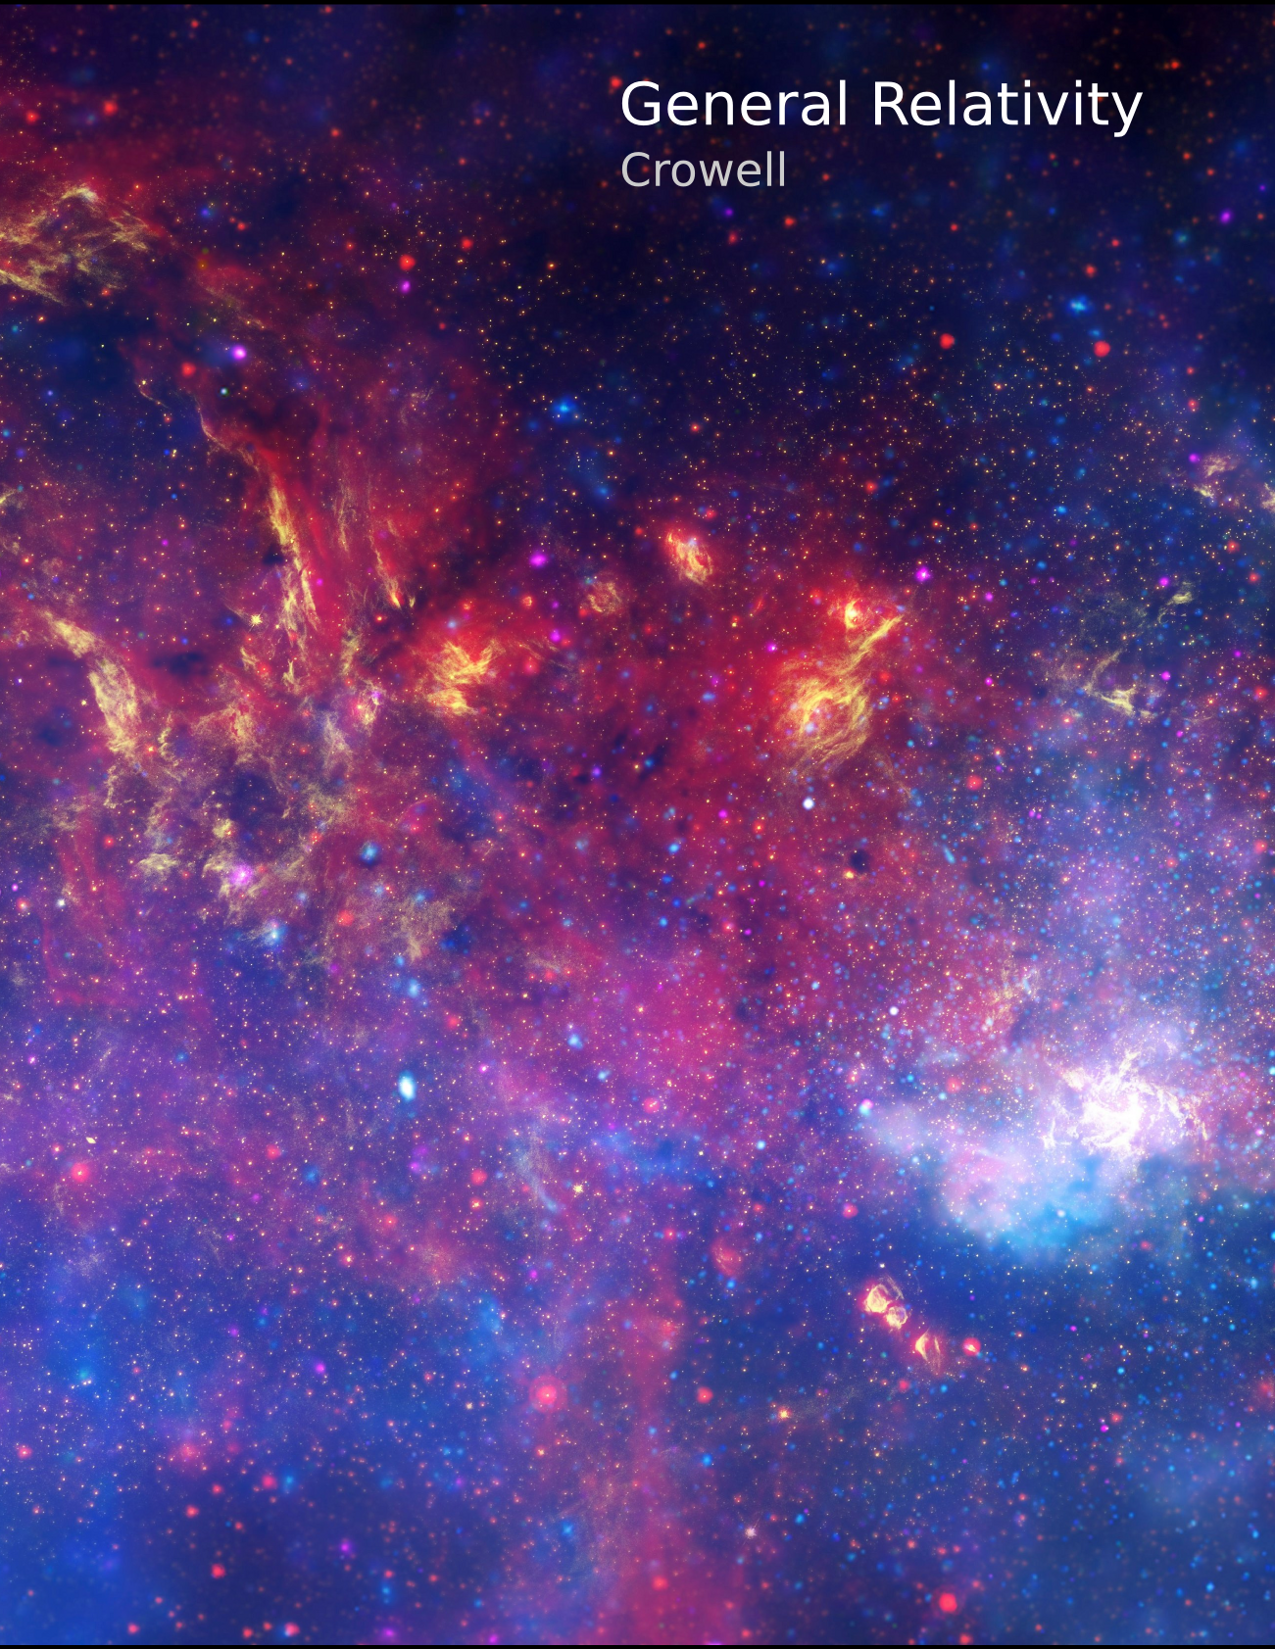
\includegraphics{cover/cover-for-pdf.png}\\
}
}%
\\


\cleardoublepage

\thispagestyle{empty}

\vspace{100mm}

{\sffamily

\noindent {\Huge General Relativity}

\noindent Benjamin Crowell

\noindent www.lightandmatter.com

}


\thispagestyle{empty}

\vspace{100mm}

\noindent
\includegraphics{cover/lmlogo}\\
Fullerton, California\\
www.lightandmatter.com

\vspace{20mm}
\noindent
Copyright \copyright  2009 Benjamin Crowell

\vspace{20mm}
\noindent
rev. \today{}

\vspace{6mm}
\noindent
Permission is granted to copy, distribute and/or modify this
document under the terms of the Creative Commons Attribution
Share-Alike License, which can be found at creativecommons.org. The license
applies to the entire text of this book, plus all the illustrations
that are by Benjamin Crowell. All the illustrations are by Benjamin
Crowell except as noted in the photo credits or in parentheses
in the caption of the figure.
This book can be downloaded free of charge
from www.lightandmatter.com in a variety of formats,
including editable formats.


\pagebreak\vspace{100mm}

\hbox{}\noindent\huge\bfseries\sffamily{}\hspace{-2mm}\ \ Brief Contents\\
\hspace{-20mm}\noindent\mynormaltype\Large\sffamily{}\begin{tabular}{rl}
\input{brief-toc.tex}
\end{tabular}
\mynormaltype

\vspace{100mm}\pagebreak

\cleardoublepage

\noindent\huge\bfseries\sffamily{}\hspace{-2mm}\ \ Contents\\
\mynormaltype

\tableofcontents

\vspace{5mm}

\noindent {\noindent
{\sffamily{} Appendix \ref{einstein-papers}: Excerpts from three papers by Einstein \dotfill \pageref{einstein-papers}}\\
``On the electrodynamics of moving bodies'' \dotfill \pageref{einstein-relativity}\\
``Does the inertia of a body depend upon its energy content?'' \dotfill \pageref{einstein-paper-mc2}\\
``The foundation of the general theory of relativity'' \dotfill \pageref{einstein-foundation}\\
{\sffamily{} Appendix \ref{hwansappendix}: Hints and solutions                      \dotfill \pageref{hwansappendix}}
}

%========================= main matter =========================
\mainmatter
%-- I want the whole book numbered sequentially, arabic:
  \pagenumbering{arabic} 
  \addtocounter{page}{10} 
\parafmt
\myeqnspacing % Do this early and often, since it gets reset by \normalsize
%========================= chapters =========================
	\renewcommand{\chapdir}{ch01}\include{ch01/ch01temp}
	\renewcommand{\chapdir}{ch02}\include{ch02/ch02temp}
	\renewcommand{\chapdir}{ch03}\include{ch03/ch03temp}
	\renewcommand{\chapdir}{ch04}\include{ch04/ch04temp}
	\renewcommand{\chapdir}{ch05}\include{ch05/ch05temp}
	\renewcommand{\chapdir}{ch06}\include{ch06/ch06temp}
	\renewcommand{\chapdir}{ch07}\include{ch07/ch07temp}
	\renewcommand{\chapdir}{ch08}\include{ch08/ch08temp}
	\formatchtoc{\large}{\quad\contentspage}{4mm} % This has to go before the last chapter.
	\renewcommand{\chapdir}{ch09}\include{ch09/ch09temp}

%=================================================================================================================================

\backmatter
\nomarginlayout   
\formatchtoc{\large}{\quad\contentspage}{0mm} % This has to go before first appendix.
\renewcommand{\chaptermark}[1]%
    {\markboth{\textsf{\thechapter\hspace{\myfooterspace}#1}}{}}
\blankchaptermarks
\vfill\pagebreak
% Einstein papers
        \onecolumn\include{ch99/einstein}
\vfill\pagebreak
% hw hints, answers, solutions
        \onecolumn\refstepcounter{appendixctr}\label{hwansappendix}%
\appendix\noindent\formatlikechapter{Appendix \ref{hwansappendix}: Hints and solutions}
	
%==================================================================
%==================================================================
%========================= Hints ==============================
%==================================================================
%==================================================================

\hwanssection{Hints}

\noindent\formatlikesubsection{Hints for Chapter 1}

\hwsolnhdr{tossed-clock} Apply the equivalence principle.\label{hint:tossed-clock}

%==================================================================
%==================================================================
%========================= Solutions ==============================
%==================================================================
%==================================================================

\hwanssection{Solutions to Selected Homework Problems}

\beginsolutions{1}

\hwsolnhdr{ordered-geom-finite-models}

Pick two points P1 and P2. By O2, there is another point P3 that is distinct
from P1 and P2. (Recall that the notation [ABC] was defined so that all three
points must be distinct.) Applying O2 again, there must be a further point
P4 out beyond P3, and by O3 this can't be the same as P1. Continuing in this
way, we can produce as many points as there are integers.

\hwsolnhdr{have-spacesuit}

(a) If the violation of (1) is tiny, then of course Kip won't really have any
practical way to violate (2), but the idea here is just to illustrate the
idea, so to make things easy, let's imagine an unrealistically large violation
of (1). Suppose that neutrons have about the same inertial mass as protons, but
zero gravitational mass, in extreme violation of (1). This implies that neutron-rich
elements like uranium would have a much lower gravitational acceleration on earth
than ones like oxygen that are roughly 50-50 mixtures of neutrons and protons.
Let's also simplify by making a second unrealistically extreme assumption: let's
say  that Kip has a keychain in his pocket made of neutronium, a substance composed of
pure neutrons. On earth, the keychain hovers in mid-air. Now he can release
his keychain in the prison cell. If he's on a planet, it will hover.
If he's in an accelerating spaceship, then the keychain will follow Newton's
first law (its tendency to do so being measured by its nonzero inertial mass),
while the deck of the ship accelerates up to hit it.

(b) It violates O1. O1 says that objects prepared in identical inertial states
(as defined by two successive events in their motion) are predicted to have
identical motion in the future. This fails in the case where Kip releases the
neutronium keychain side by side with a penny.

\hwsolnhdr{tossed-clock}
By the equivalence principle, we can adopt a frame tied to the tossed clock, B, and in this
frame there is no gravitational field. We see a desk and clock A go by. The desk applies
a force to clock A, decelerating it and then reaccelerating it so that it comes back.
We've already established that the effect of motion is to slow down time, so clock
A reads a smaller time interval.

\hwsolnhdr{clock-at-center-of-earth}
(a) Generalizing the expression $gy/c^2$ for the fractional time dilation to the case of a nonuniform
field, we find $\Phi/c^2$, where $\Phi$ is the Newtonian gravitational potential, i.e., the
gravitational energy per unit mass.
The shell theorem gives a gravitational field $g=Mr/R^3$. Integration shows
$\Phi=Mr^2/2R^3$. The difference in the gravitational potential between these two points, divided by $c^2$, is
$\Phi/c^2=M/2c^2R$, which comes out to be $3.5\times 10^{-10}$. This is the fractional difference in clock rates.
% calc -x -e "M=5.97 10^24 kg; R=6370 km; GM/(2c^2R)"
(b) The probe's velocity is on the same order of magnitude as escape velocity from the inner solar system,
so very roughly we can say that $v\sim\sqrt{|\Delta\Phi|}$, where $\Delta\Phi$ is the difference between the gravitational
potential at the earth's orbit and infinity. This gives a Doppler shift $v/c\sim \sqrt{|\Delta\Phi|}/c$.
We saw in part a that the gravitational Doppler shift was $\Delta\Phi/c^2$, which is the square of this
quantity, and therefore much smaller.

\hwsolnhdr{ep-charge}
(a) In case 1 there is no source of energy, so the particle cannot radiate.
In case 2-4, the particle radiates, because there are sources of energy (loss of
gravitational energy in 2 and 3, the rocket fuel in 4).

(b) In 1, Newton says the object is subject to zero net force, so its motion
is inertial. In 2-4, he says the object is subject to a nonvanishing net force,
so its motion is noninertial. This matches up with the results of the energy analysis.

(c) The equivalence principle, as discussed on page \pageref{sec:chiao-paradox},
is vague, and is particularly difficult to apply successful and unambiguously to
situations involving electrically charged objects, due to the difficulty of
defining locality. Applying the equivalence principle in the most naive way,
we predict that there can be no radiation in cases 2 and 3 (because the object is
following a geodesic, minding its own business).
In case 4, everyone agrees that there will be radiation observable back on earth
(although it's possible that it would not be observable to an observer momentarily
matching velocities with the rocket).
The naive equivalence principle says that 1 and 4 must give the same result, so
we should have radiation in 1 as well. These predictions are wrong in two out of
the four equations, which tells us that we had better either not apply the equivalence
principle to charged objects, or not apply it in such a naive way.

\hwsolnhdr{dewitt-estimate}

(a) The dominant form of radiation from the orbiting charge will be the lowest-order
nonvanishing multipole, which in this case is a dipole. The power radiated from
a dipole scales like $d^2\omega^4$, where $d$ is the dipole moment. For an orbit of
radius $r$, this becomes $q^2r^2\omega^4$. To find the reaction force on the charged particle,
we can use the relation $p=E/c$ for electromagnetic waves (section \ref{subsec:gravitational-redshifts}),
which tells us that the force is equal to the power, up to a proportionality constant $c$.
Therefore $a_r\propto q^2r^2\omega^4/m$. The gravitational acceleration is $a_g=\omega^2 r$,
so we have $a_r/a_g \propto (q^2/m)\omega^2 r$, or $a_r/a_g \propto (q^2/m)a_g$, where the
$a_g$ on the right can be taken as an orbital parameter, and for a low-earth orbit is very nearly equal to
the usual acceleration of gravity at the earth's surface.

(b) In SI units, $a_r/a_g \sim (k/c^4)(q^2/m)a_g$, where $k$ is the Coulomb constant.

(c) The result is $10^{-34}$. If one tried to do this experiment in reality, the effect would be
impossible to detect, because the proton would be affected much more strongly by ambient electric and
magnetic fields than by the effect we've calculated.

Remark: It is odd that the result depends on $q^2/m$, rather than on the charge-to-mass ratio $q/m$,
as is usually the case for a test particle's trajectory. This means that we get a different answer
if we take two identical objects, place them side by side, and consider them as one big object! This is not as unphysical
as it sounds. The two side-by-side objects radiate coherently, so the field they radiate is doubled, and the
radiated power is quadrupled. Each object's rate of orbital decay is doubled, with the extra effect coming
from electromagnetic interactions with the other object's fields.

\beginsolutions{2}

\hwsolnhdr{clock-postulate}

(a) Let $t$ be the time taken in the lab frame for the light to go from one mirror to the other,
and $t'$ the corresponding interval in the clock's frame. Then $t'=L$, and $(vt)^2+L^2=t^2$,
where the use of the same $L$ in both equations makes use of our prior knowledge that there
is no transverse length contraction.
Eliminating $L$, we find the expected expression for $\gamma$, which is independent of $L$
(b) If the result of a were independent of $L$, then the relativistic time dilation would depend
on the details of the construction of the clock measuring the time dilation. We would be forced
to abandon the geometrical interpretation of special relativity.
(c) The effect is to replace $vt$ with $vt+at^2/2$ as the quantity inside the parentheses
in the expression $(\ldots)^2+L^2=t^2$. The resulting correction terms are of higher order in
$t$ than the ones appearing in the original expression, and can therefore be made as small
in relative size as desired by shortening the time $t$. But this is exactly what happens when
we make the clock sufficiently small.

\hwsolnhdr{mountain-valley}

Since gravitational redshifts can be interpreted as gravitational time dilations, the gravitational
time dilation is given by the difference in gravitational potential $g\der r$ (in units where $c=1$).
The kinematic effect is given by $\der\gamma=\der(v^2)/2=\omega^2 r \der r$. The ratio of the
two effects is $\omega^2 R \cos\lambda/g$, where $R$ is the radius of the Earth and $\lambda$ is the
latitude. Tokyo is at 36 degrees latitude, and plugging this in gives the claimed result.

\hwsolnhdr{sagnac-area}

(a) Reinterpret figure \figref{thomas-as-area} on p.~\pageref{fig:thomas-as-area} as a picture of a Sagnac
ring interferometer. Let light waves 1 and 2 move around the loop in opposite senses. Wave 1 takes time
$t_{1i}$ to move inward along the crack, and time $t_{1o}$ to come back out. Wave 2 takes times
$t_{2i}$ and $t_{2o}$. But $t_{1i}=t_{2i}$ (since the two world-lines are identical), and similarly
$t_{1o}=t_{2o}$. Therefore creating the crack has no effect on the interference between 1 and 2,
and splitting the big loop into two smaller loops merely splits the total phase shift between them.
(b) For a circular loop of radius $r$, the time of flight of each wave is proportional to $r$, and
in this time, each point on the circumference of the rotating interferometer travels a distance
$v(\text{time})=(\omega r)(\text{time})\propto r^2$. (c) The effect is proportional to area, and
the area is zero. (d) The light clock in c has its two ends synchronized according to the Einstein
prescription, and the success of this synchronization verifies Einstein's assumption of commutativity
in this particular case. If we make a Sagnac interferometer in the shape of a triangle, then the Sagnac
effect measures the failure of Einstein's assumption that all three corners can be synchronized
with one another.

\hwsolnhdr{velocity-addition-matrix-taylor}

Here is the program:
\begin{listing}{1}
L1:matrix([cosh(h1),sinh(h1)],[sinh(h1),cosh(h1)]);
L2:matrix([cosh(h2),sinh(h2)],[sinh(h2),cosh(h2)]);
T:L1.L2;
taylor(taylor(T,h1,0,2),h2,0,2);
\end{listing}
The diagonal components of the result are both $1+\eta_1^2/2+\eta_2^2/2+\eta_1\eta_2+\ldots$
Everything after the 1 is nonclassical. The 
off-diagonal components are $\eta_1+\eta_2+\eta_1\eta_2^2/2+\eta_2\eta_1^2/2+\ldots$,
with the third-order terms being nonclassical.

\beginsolutions{3}

\hwsolnhdr{cylinder-spacetime}

(a) As discussed in example \ref{eg:extrinsic-curvature} on page \pageref{eg:extrinsic-curvature}, a cylinder has local,
intrinsic properties identical to those of flat space. The cylindrical model therefore has the same properties L1-L5
as our standard model of Lorentzian space, provided that L1-L5 are taken as purely local statements.

(b) The cylindrical model does violate L3. In this model, the doubly-intersecting world-lines
described by property G will not occur if the world-lines are oriented exactly parallel to the cylinder. This picks
out a preferred direction in space, violating L3 if L3 is interpreted globally. Frames moving parallel to the axis have
different properties from frames moving perpendicular to the axis.

But just because this particular model violates the
global interpretation of L3, that doesn't mean that all models of G violate it. We could instead construct a model in
which space wraps around in every direction. In the 2+1-dimensional case, we can visualize the spatial part of such a model as the surface
of a doughnut embedded in three-space, with the caveat that we don't want to think of the doughnut hole's circumference as being
shorter than the doughnut's outer radius. Giving up the idea of a visualizable model embedded in a higher-dimensional space,
we can simply take a three-dimensional cube and identify its opposite faces. Does this model violate L3? It's not quite as
obvious, but actually it does. The spacelike great-circle geodesics of this model come in different circumferences, with the shortest
being those parallel to the cube's axes.

We can't prove by constructing a finite number of models that every possible model of G violates L3. The two models we've found, however,
can make us suspect that this is true, and can give us insight into how to prove it. For any pair of world-lines that
provide an example of G, we can fix a coordinate system K in which the two particles started out at A by flying off back-to-back.
In this coordinate system, we can measure the sum of the distances traversed by the two particles from A to B. (If homegeneity, L1,
holds, then they make equal contributions to this sum.) The fact that the world-lines were traversed by material particles
means that we can, at least in principle, visit every point on them and measure the total distance using rigid rulers.
We call this the circumference of the great circle AB, as measured in a particular frame.
The set of all such circumferences has some greatest lower bound. If this bound is zero, then such geodesics can exist locally, and
this would violate even the local interpretation of L1-L5. If the bound is nonzero, then let's fix a circle that has
this minimum circumference. Mark the spatial points this circle passes through, in the frame of reference defined above.
This set of points is a spacelike circle of minimum radius. Near a given point on the circle, the circle looks like
a perfectly straight axis, whose orientation is presumably random. Now let some observer $\zu{K}'$ travel around this circle at a velocity
$v$ relative to K, measuring the circumference with a Lorentz-contracted ruler. The circumference is greater than the minimal
one measured by K. Therefore for any axis with a randomly chosen orientation, we have a preferred rest frame in which the
corresponding great circle has minimum circumference. This violates L3. Thanks to physicsforums user atyy for suggesting this
argument.

More detailed discussions of these issues are given in Bansal et al., \url{arxiv.org/abs/gr-qc/0503070v1},
and Barrow and Levin, \url{arxiv.org/abs/gr-qc/0101014v1}.

\hwsolnhdr{lorentz-si}

In these Cartesian coordinates, the metric is diagonal and has elements with opposite signs.
Due to the SI units, it is not possible for the two nonzero elements of the metric to have the
same units. Let's arbitrarily fix $g_{tt}=1$. Then we must have $g_{xx}=c^{-2}$. Using the metric to
lower the index on $\der s^a$, we find $\der s_a = (\der s^t,c^{-2} \der s^x)$.

\hwsolnhdr{contraction-of-metric}

According to the Einstein summation convention, the repeated index implies a sum, so the result is
a scalar. As shown in
example \ref{eg:mixed-metric} on p.~\pageref{eg:mixed-metric}, each term in the sum equals 1, so
the result is unitless and simply equals the number of dimensions.

\hwsolnhdr{ungrammatical}

(a) The first two violate the rule that summation only occurs over up-down pairs of indices.
The third expression would result in a quantity that couldn't be classified as either contravariant
or covariant. (b) In differential geometry, different elements of the same tensor can have different
units. Since, as remarked in the problem, $U_{aa}$ were to be interpreted as a sum, this mean adding things
that had different units. In the expression $p^a-q_a$, even if we suppose that $p$ and $q$ both represent
the same type of physical quantity, e.g., force, their covariant and contravariant versions would
not necessarily have the same units unless we happened to be working in coordinates such that the
metric was unitless.

\hwsolnhdr{lat-lon-force}

Assuming the mountaineer uses radians and the metric system, the coordinates have units
1, 1, and m (where 1 means a unitless quantity and m means meters --- radians are not really units).
Therefore the units of an infinitesimal difference in coordinates $\der s^a$ are
also $(1,1,\munit)$. Because the coordinates are orthogonal, the metric is diagonal.
If we want $g_{ab}\der s^a \der s^b$ to have units of $\munit^2$, then its diagonal elements
must have units of $(\munit^2,\munit^2,1)$.
%
The upper-index metric $g^{ab}$ is the inverse of its lower-index version $g_{ab}$, so its units are
$(\munit^{-2},\munit^{-2},1)$.
%
Mechanical work has units of $\nunit\cdot\munit$,
so given $\der W=F_a \der s^a$, the units of $F_a$ must be $(\nunit\cdot\munit,\nunit\cdot\munit,\nunit)$.
%
Raising the index on the force
using $g^{ab}$ gives $(\nunit/\munit,\nunit/\munit,\nunit)$.

\hwsolnhdr{burke-three-d}

The only aspect of the geometrical representation that needs to be changed is that instead of
representing an upper-index vector using a pair of parallel lines, we should use a pair of parallel planes.

\hwsolnhdr{gps-t-discontinuity}

The coordinate $T$ would have a discontinuity of $2\pi\omega r^2/(1-\omega^2 r^2)$. Reinserting factors of $c$ to make it work
out in SI units, we have $2\pi\omega r^2 c^{-2}/(1-\omega^2 r^2 c^{-2}) \approx 207\ \zu{ns}$. The exact error in position that
would result is dependent on the geometry of the current position of the satellites, but it would be on the order of $c\Delta T$,
which is $\sim 100\ \munit$. This is considerably worse than civilian GPS's 20-meter error bars.

\hwsolnhdr{carousel-paradox}

The process that led from the Euclidean metric of example \ref{eg:metric-in-polar-coords} on page \pageref{eg:metric-in-polar-coords}
to the non-Euclidean one of equation [\ref{eq:rotating-spatial}] on page \pageref{eq:rotating-spatial} was not just a series
of coordinate transformations. At the final step, we got rid of the variable $t$, reducing the number of dimensions by one.
Similarly, we could take a Euclidean three-dimensional space and eliminate all the points except for the ones on the surface
of the unit sphere; the geometry of the embedded sphere is non-Euclidean, because we've redefined geodesics to be lines that
are ``as straight as they can be'' (i.e., have minimum length) while restricted to the sphere. In the example of the carousel, the final step effectively
redefines geodesics so that they have minimal length as determined by a chain of radar measurements.

\hwsolnhdr{carousel-metric}

(a) No.
The track is straight in the lab frame, but curved in the
rotating frame. Since the spatial metric in the rotating frame is symmetric with respect to clockwise and counterclockwise,
the metric can never result in geodesics with a specific handedness.
(b) The $\der\theta'^2$ term of the metric blows up here. A geodesic connecting point A, at $r=1/\omega$, with point B, at $r<1/\omega$,
must have minimum length. This requires that the geodesic be directly radial at A, so that $\der\theta'=0$; for if not, then we could
vary the curve slightly so as to reduce $|\der\theta'|$, and the resulting increase in the $\der r^2$ term would be negligible
compared to the decrease in the $\der\theta'^2$ term. (c) No. As we found in part a, laser beams can't be used to form geodesics.

\hwsolnhdr{penrose-generalization}
A and B are equivalent under a Lorentz transformation, so the Penrose result clearly includes B. The outline of the sphere is still spherical.
C is also equivalent to A and B, because there are only two effects (Lorentz contraction and optical aberration), and both of
them depend only on the observer's instantaneous velocity, not on his history of motion.
D is not a well-defined question. When asking this question, we're implicitly assuming that the sphere has some
``real'' shape, which appears different because the sphere has been set into motion. But
you can't impart an angular acceleration to a perfectly rigid body in relativity.

\hwsolnhdr{dispersion}
Applying the de Broglie relations to the relativistic identity $m^2=E^2-p^2$, we find the
dispersion relation to be $m^2=\omega^2-k^2$. The group velocity is $\der\omega/\der k=\sqrt{1-(m/\omega)^2}$.
Applying the de Broglie relations to this, and associating the group velocity with $v$, we have
$v=\sqrt{1-(m/E)^2}$, which is equivalent to $E=m\gamma$. Since $E=m\gamma$ has been established,
and $m^2=E^2-p^2$ was assumed, it follows immediately that $p=m\gamma v$ holds as well.
All hell breaks loose if we try to associate $v$ with the phase velocity, which is
$\omega/k=\sqrt{1+(m/k)^2}$. For example, the phase velocity is always greater than $c(=1)$ for $m>0$.

\beginsolutions{4}

\hwsolnhdr{photon-four-velocity}

The four-velocity of a photon (or of any massless particle) is undefined.
One way to see this is that $\der\tau=0$ for a massless particle, so $v^i=\der x^i/\der\tau$
involves division by zero. Alternatively, $p^i=mv^i$ would always give an energy and momentum
of zero if $v^i$ were well defined, yet we know that massless particles can have both energy and momentum.

\hwsolnhdr{lhc-proton-speed}

To avoid loss of precision in numerical operations like subtracting $v$ from $1$,
it's better to derive an ultrarelativistic approximation. The velocity corresponding
to a given $\gamma$ is $v=\sqrt{1-\gamma^{-2}}\approx 1-1/2\gamma^2$, so
$1-v\approx 1/2\gamma^2=(m/E)^2/2$. Reinserting factors of $c$ so as to make the units
come out right in the SI system, this becomes $(mc^2/E)^2/2=9\times 10^{-9}$.

\hwsolnhdr{hafele-frame-indept}

The time on the clock is given by $s=\int \der s$, where the integral is over the clock's
world-line. The quantity $\der s$ is our prototypical Lorentz scalar, so it's frame-independent.
An integral is just a sum, and the tensor transformation laws are linear, so the integral of
a Lorentz scalar is still a Lorentz scalar. Therefore $s$ is frame-independent. There is
no requirement that we use an inertial frame. It would also work fine, for example, in a frame
rotating with the earth. We don't even need to have a frame of reference.
All of the above applies equally well to any
coordinate system at all, even one that doesn't have any sensible interpretation as some
observer's frame of reference.

\hwsolnhdr{dirac-sea-invariant}

Such a transformation would take an energy-momentum four-vector $(E,\vc{p})$, with $E>0$, to
a different four-vector $(E',\vc{p}')$, with $E'<0$. That transformation would also have the
effect of transforming a timelike displacement vector from the future light cone to the past
light cone. But the Lorentz transformations were specifically constructed so as to preserve
causality (property L5 on p.~\pageref{sec:lorentz-geometry}), so this can't happen.

\hwsolnhdr{doppler-three-d}

A spatial plane is determined by the light's direction of propagation and the relative velocity
of the source and observer, so the 3+1 case reduces without loss of generality to 2+1 dimensions.
The frequency four-vector must be lightlike, so its most general possible form is
$(f,f\cos\theta,f\sin\theta)$, where $\theta$ is interpreted as the angle between the direction of
propagation and the relative velocity. Putting this through a Lorentz boost along the $x$ axis,
we find $f'=\gamma f(1+v\cos\theta)$, which agrees with Einstein's equation on page
\pageref{einstein-doppler}, except for the arbitrary convention involved in defining the sign of $v$.

\hwsolnhdr{classical-electron-radius}

The exact result depends on how one assumes the charge is distributed, so this can't be any more than a rough
estimate. The energy density is $(1/8\pi k)E^2 \sim ke^2/r^4$, so the total energy is an integral of the form
$\int r^{-4} \der V \sim \int r^{-2} \der r$, which diverges like $1/r$ as the lower limit of integration approaches
zero. This tells us that most of the energy is at small values of $r$, so to a rough approximation we can just
take the volume of integration to be $r^3$ and multiply by a fixed energy density of $ke^2/r^4$. This gives
an energy of $\sim ke^2/r$. Setting this equal to $mc^2$ and solving for $r$, we find $r \sim ke^2/mc^2 \sim 10^{-15}\ \munit$.

Remark: Since experiments have shown that electrons do \emph{not} have internal structure on this scale, we conclude that
quantum-mechanical effects must prevent the energy from blowing up as $r\rightarrow 0$.

\hwsolnhdr{galilean-em}

Doing a transformation first by $\vc{u}$ and then by $\vc{v}$ results in
$\vc{E}''=\vc{E}-\vc{v}\times(\vc{u}\times\vc{E})+(\vc{u}+\vc{v})\times\vc{B}$. This is not of the same
form, because if $\vc{B}=0$, we can have $\vc{E}''\ne\vc{E}$.

\beginsolutions{5}

\hwsolnhdr{christoffel-rescale-metric}
The equation for the Christoffel symbols in terms of the metric was
\begin{equation*}
  \Gamma\indices{^c_{ab}} = \frac{1}{2}g^{cd}\left(\partial_a g_{bd}+\partial_b g_{ad}-\partial_d g_{ab}\right)\eqquad.
\end{equation*}
Because both the metric matrix and its inverse appear, we get factors of $\alpha$ and
$1/\alpha$ that cancel out. Therefore there is no effect on the Christoffel symbols or
on the geodesics. This certainly makes sense in the case of $\alpha=-1$, because this
is just a change in the choice of signature, which is an arbitrary convention. It
also makes sense that rescaling the metric by a nonzero positive factor has no effect
on the geodesics --- we would expect this to change the measurement of geodesics, but we
would not expect it to make different curves be geodesics.



\hwsolnhdr{taub-christoffel}

The inverse metric has $g^{tt}=t$ and $g^{\theta\theta}=-1/t$.
The nonvanishing symbols are:
\begin{align*}
  \Gamma\indices{^t_{tt}} &= \frac{1}{2}g^{tt}(\partial_t g_{tt}+\partial_t g_{tt}-\partial_t g_{tt}) = -1/2t\\
  \Gamma\indices{^t_{\theta\theta}} &= \frac{1}{2}g^{tt}(\partial_t g_{\theta\theta}) = t/2  \\
  \Gamma\indices{^\theta_{\theta t}} &= \Gamma\indices{^\theta_{\theta t}} = \frac{1}{2}g^{\theta\theta}(\partial_t g_{\theta\theta}) = 1/2t  \\
\end{align*}

\hwsolnhdr{uniform-field}

(a) Expanding in a Taylor series, they both have $g_{tt}=1+2gz+\ldots$

(b) This property holds for [\ref{eq:uniform-field-metric-rindler}] automatically because of the way it was constructed.
In [\ref{eq:uniform-field-metric-exp}], the nonvanishing Christoffel
symbols (ignoring permutations of the lower indices) are $\Gamma\indices{^t_{zt}}=g$ and $\Gamma\indices{^z_{tt}}=ge^{2gz}$.
We can apply the geodesic equation with the affine parameter taken to be the proper time, and this gives 
$\ddot{z}=-ge^{2gz}\dot{t}^2$, where dots represent differentiation with respect to proper time.
For a particle instantaneously at rest, $\dot{t}=1/\sqrt{g_{tt}}=e^{-2gz}$, so $\ddot{z}=-g$.

(c) [\ref{eq:uniform-field-metric-rindler}] was constructed by performing a change of coordinates on a flat-space metric, so it is flat. 
The Riemann tensor of [\ref{eq:uniform-field-metric-exp}] has $R\indices{^t_{ztz}}=-g^2$, so [\ref{eq:uniform-field-metric-exp}] isn't flat.
Therefore the two can't be the same under a change of coordinates.

(d) [\ref{eq:uniform-field-metric-rindler}] is flat, so its curvature is constant. [\ref{eq:uniform-field-metric-exp}] has the
property that under the transformation $z\rightarrow z+c$, where $c$ is a constant, the only change is a rescaling of the
time coordinate; by coordinate invariance, such a rescaling is unobservable.

\hwsolnhdr{closed-and-open}
(a) $0 \le x \le 1$\\
(b) $0 \le x < 1$\\
(c) $x^2 \le 2$

\hwsolnhdr{double-cone-not-manifold}
The double cone fails to satisfy axiom M2, because the apex has properties that differ topologically from those of
other points: deleting it chops the space into two disconnected pieces.

\hwsolnhdr{torus-is-manifold}
When we use a word like ``torus,'' there is some hidden ambiguity. We could mean something strange like the following. Suppose
we construct the three-dimensional space of coordinates $(x,y,z)$ in which all three coordinates are rational numbers. Then let
a torus be the set of all such points lying at a distance of 1/2 from the nearest point on a unit circle. This is in some sense
a torus, but it doesn't have the topological properties one usually assumes. For example, two continuous curves on its surface can cross
without having a point of intersection. We can't get anywhere without assuming that the word ``torus'' refers to a surface that
has the usual topological properties.

Now let's prove that it's a manifold using both definitions.

Using the topological definition, M1 is satisfied with $n=2$, because every point on the
surface lives in a two-dimensional neighborhood. M2 holds because the only differences between points are those that are not
topological, e.g., Gaussian curvature. M3 holds due to the interpretation outlined in the first paragraph.

Alternatively, we can use the local-coordinate definition. We have already shown that a circle
is a 1-manifold, which can be coordinatized in two patches by an angle $\phi$. The torus can therefore be coordinatized by
a pair of such angles, $(\phi_1,\phi_2)$, in four patches. Again we need to assume the interpretation given above, since
otherwise real-number pairs like $(\phi_1,\phi_2)$ wouldn't have the same topology as points on the rational-number torus.

\hwsolnhdr{sphere-not-homeomorphic-to-torus}
In the torus, we can construct a closed curve C that encircles the hole. If we have a homeomorphism, C must have
an image $\zu{C}'$ under that homeomorphism that is a closed curve in the sphere.  $\zu{C}'$ can then be
contracted continuously to a point, and since the inverse of the homeomorphism is also continuous, it would be
possible to contract C continuously to a point. But this is impossible because C encircles the hole.

\hwsolnhdr{nontrivial-curvature-in-one-plus-one}
(a) The Christoffel symbols are (assuming I didn't make a mistake in calculating them by
hand) $\Gamma^t_{xx}=(1/2)pt^{p-1}$ and $\Gamma^x_{xt}=\Gamma^x_{tx}=(1/2)pt^{-1}$.
(b) After that, I resorted to a computer algebra system (Maxima), which told me that, for example,
the Ricci tensor has $R_{tt}=(p/2-p^2/4)t^{-2}$.

\hwsolnhdr{gaussian-curvature-at-edge}

The answer to this is a little subtle, since it depends on how we take the limit.
Suppose we join two planes with a section of a cylinder having radius $\rho$, and let $\rho$ go to zero.
The Gaussian curvature of a cylinder is zero, so in this limit we fail to reproduce the correct result.
On the other hand, suppose we take a discus of radius $\rho_1$ whose edge has a curve of radius $\rho_2$.
in the limit $\rho_1\rightarrow+\infty$, $\rho_2\rightarrow0^+$, we can get either $K=1/(\rho_1\rho_2)\rightarrow 0$ or
$K\rightarrow+\infty$, depending on how quickly $\rho_1$ and $\rho_2$ approach their limits.

\beginsolutions{6}

\hwsolnhdr{black-hole-slingshot}
(a) In the center of mass frame, symmetry guarantees that the test particle exits with a
 speed equal to the speed with which it entered, and
 the entry and exit velocities are $v$ and $-v$. Now let's switch to the sun's frame. This
 involves adding $u$ to all velocities, so the entry and exit velocities become $v+u$ and $-v+u$.
 The difference in speed is $2u$.

(b) The derivation assumed that velocities add linearly when you change frames of reference, which is a nonrelativistic
 approximation. Relativistically, velocities combine not like $u+v$ but like $(u+v)/(1+uv)$.
 If you put in $v=1$, the result for the combined velocity is always 1.

This is a funny case where we can get the answer to a gravitational problem purely through special relativity. 
We might worry that the SR-based answer is wrong, because we really need GR for gravity. But we can get the
 same answer from GR, since GR says that a test particle always follows a geodesic, and a lightlike geodesic always
 remains lightlike. The reason SR worked is that an observer could watch a patch of flat space far away from the
 black hole, observe a wave-packet of light passing through that patch on the way to the black hole, and
 then observe it again on the way back out. Since the patch is flat, SR works.

\hwsolnhdr{impact-in-finite-proper-time}
(a) $L=0$ by symmetry. The quantity $E$ can be interpreted as the energy per unit mass that is added to the entire
system by inserting the test particle. Since the test particle starts at rest and far away, the added energy is
simply the mass of the particle, and $E=1$.

(b) In the special case $L=0$, $E=1$,
the general equation of motion for a test particle in a Schwarzschild spacetime
becomes simply $\dot{r}^2 = 2m/r$. Separating variables and integrating, we have $r \propto s^{2/3}$,
where the constant of integration is chosen to be zero. This clearly shows that we move from any given
$r$ to $r=0$ in a finite proper time $s$.

\hwsolnhdr{astroid}
(a) For a displacement with $\der\phi=0$, we have $\der s^2=g_{tt}\der t^2$, so
$g_{tt}=\sqrt{\der s/\der t}=\sqrt{3\sin t\cos t}$. For an azimuthal displacement,
$\der s= y\der\phi$, so $g_{\phi\phi}=\sqrt{y}=\sin^{3/2}t$.\\
(b) At places on the surface of revolution corresponding to the cusps of the astroid, one or
both of the lower-index elements of the metric go to zero, which means that the corresponding
upper-index elements blow up. These are the sharp points of the surface at the $x$ axis and
the sharp edge at its waist. There are at least coordinate singularities there, but the question
is whether they are intrinsic. The only intrinsic measure of curvature in two dimensions is the Gaussian
curvature, which can be interpreted as (minus) the product of the curvatures along the two principal axes,
here $k_1=-(2/3)\csc 2t$ and $k_2=1/y=\sin^{-3} t$. At the waist, both factors blow up, so the
Gaussian curvature, which is intrinsic, blows up, and this is not just a coordinate singularity.
The same thing happens at the tips. Interestingly, a geodesic that hits one of these singularities can still be
traced through in a continuous way and extended onward such that its arc length remains finite. This property is
called geodesic completeness.\index{geodesic completeness}\index{completeness!geodesic}\index{manifold!geodesically complete}

\hwsolnhdr{carousel-singularities} 
(a) There are singularities at $r=0$, where $g_{\theta'\theta'}=0$, and $r=1/\omega$,
where $g_{tt}=0$. These are considered singularities because the inverse of the metric
blows up. They're coordinate singularities, because they can be removed by a change of
coordinates back to the original non-rotating frame.\\
(b) This one has singularities in
the same places. The one at $r=0$ is a coordinate singularity, because at small $r$
the $\omega$ dependence is negligible, and the metric is simply that of ordinary
plane polar coordinates in flat space. The one at $r=1/\omega$ is not a coordinate
singularity. The following Maxima code calculates its scalar curvature $R=R\indices{^a_a}$,
which is esentially just the Gaussian curvature, since this is a two-dimensional space.
\begin{listing}{1}
load(ctensor);
dim:2;
ct_coords:[r,theta];
lg:matrix([-1,0],
          [0,-r^2/(1-w^2*r^2)]);
cmetric();   
ricci(true);
scurvature();
\end{listing}
% carousel-singularities.mac
The result is $R=6\omega^2/(1-2\omega^2r^2+\omega^4r^4)$.
This blows up at $r=1/\omega$, which shows that this is not a coordinate
singularity. The fact that $R$ does not blow up at $r=0$ is consistent with our
earlier conclusion that $r=0$ is a coordinate singularity, but would not have been
sufficient to prove that conclusion.\\
(c) The argument is incorrect. The Gaussian curvature is not just proportional to
the angular deficit $\epsilon$, it is proportional to the
limit of $\epsilon/A$, where $A$ is the area of the triangle. The area of the triangle
can be small, so there is no upper bound on the ratio $\epsilon/A$.
Debunking the argument restores consistency with the answer to part b.

\hwsolnhdr{slowdown-curvature}
The only nonvanishing Christoffel symbol is $\Gamma\indices{^t_{tt}}=-1/2t$. The antisymmetric
treatment of the indices in $R\indices{^a_{bcd}} = \partial_c \Gamma\indices{^a_{db}} - \partial_d \Gamma\indices{^a_{cb}}
                        + \Gamma\indices{^a_{ce}}\Gamma\indices{^e_{db}}-\Gamma\indices{^a_{de}}\Gamma\indices{^e_{cb}}$
guarantees that the Riemann tensor must vanish when there is only one nonvanishing Christoffel symbol.

\hwsolnhdr{bogus-vacuum-field-equation}
The first thing one notices is that the equation $R_{ab}=k$ isn't written according to the usual rules of grammar
for tensor equations. The left-hand side has two lower indices, but the right-hand side has none. In the language of freshman physics,
this is like setting a vector equal to a scalar. Suppose we interpret it as meaning that each of $R$'s 16 components should equal
$k$ in a vacuum. But this still isn't satisfactory, because it violates coordinate-independence. For example, suppose we
are initially working with some coordinates $x^\mu$, and we then rescale all four of them according to $x^{\mu'}=2x^\mu$.
Then the components of $R_{ab}$ all scale down by a factor of 4. But this would violate the proposed field equation.

\hwsolnhdr{no-schwarzschild-in-three-dimensions}
The following Maxima code calculates the Ricci tensor for a metric with $g_{tt}=h$ and $g_{rr}=k$.

\begin{listing}{1}
load(ctensor);
dim:3;
ct_coords:[t,r,phi];
depends(h,r);
depends(k,r);
lg:matrix([h,0,0],
          [0,-k,0],
          [0,0,-r^2]);
cmetric();
ricci(true);
\end{listing}

\noindent Inspecting the output (not reproduced here), we see that $R_{\phi\phi}=0$ requires $k'/k=h'/h$. Since the logarithmic derivatives of $h$ and $k$ are the
same, the two functions can differ by at most a constant factor $c$. So now we do a second iteration of the calculation:

\begin{listing}{1}
load(ctensor);
dim:3;
ct_coords:[t,r,phi];
depends(h,r);
lg:matrix([h,0,0],
          [0,-c*h,0],
          [0,0,-r^2]);
cmetric();
ricci(true);
\end{listing}

\noindent The result for $R_{rr}$ is independent of $c$. Since $h$ is essentially the gravitational potential,
we have the requirements $h'>0$ (because gravity is attractive)
and $h''<0$ (because gravity weakens with distance). Therefore we find that  $R_{rr}$
is positive, and we do not obtain a vacuum solution.

\hwsolnhdr{flip-velocity-vectors}
This idea is not well defined because it implicitly assumes that we can fix a global
frame of reference. The notion of reversing velocity
vectors (i.e., reversing the spacelike components of 4-velocities) implies
that there are some velocity vectors whose spacelike parts are zero, so that
they aren't changed by a flip. This amounts to choosing a frame of reference. To
be able to do the flip globally, you'd have to have some sensible notion of
a global frame of reference, but we don't necessarily have that. (In a spacetime with closed timelike
curves, there is also the issue that we don't have complete freedom to choose initial
conditions on a spacelike surface, because these conditions might end up not being
consistent with themselves when evolved around a CTC.)

\beginsolutions{7}

\hwsolnhdr{alice-stationary}
(a) If she makes herself stationary relative to the sun, she will still experience local geometrical changes
because of the planets. (b) If it was to be impossible for her to prove the universe's nonstationarity,
then any world-line she picked would have to experience constant local geometrical conditions.
A counterexample is any world-line extending back to the Big Bang, which is a singularity with drastically
different conditions than any other region of spacetime.
(c) To maintain a constant local geometry, she would have to ``surf'' the wave, but
she can't do that, because it propagates at the speed of light. (d) There are places where the
local mass-energy density is increasing, and the field equations link this to a change in the local
geometry.

\hwsolnhdr{petrov-strength}

Under these special conditions, the geodesic equations become $\ddot{r}=\Gamma\indices{^r_{tt}}\dot{t}^2$,
$\ddot{\phi}=0$, $\ddot{t}=0$,
where the dots can in principle represent differentation with respect to any affine parameter we like, but
we intend to use the proper time $s$.
By symmetry, there will be no motion in the $z$ direction.
The Christoffel symbol equals $-(1/2)e^r(\cos\sqrt{3}r-\sqrt{3}\sin\sqrt{3}r)$. At a location where
the cosine equals 1, this is simply $-e^r/2$. For $\dot{t}$, we have $\der t/\der s=1/\sqrt{g_{tt}}=e^{-r/2}$.
The result of the calculation is simply $\ddot{r}=-1/2$, which is independent of $r$.

\hwsolnhdr{rotation-with-no-center}

The Petrov metric is one example. The metric has no singularities anywhere, so the $r$ coordinate
can be extended from $-\infty$ to $+\infty$, and there is no point that can be considered the center.
The existence of a $\der\phi \der t$ term in the metric shows that it is not static.

A simpler example is a spacetime made by taking a flat Lorentzian space and making it wrap around topologically
into a cylinder, as in problem \ref{hw:cylinder-spacetime} on p.~\pageref{hw:cylinder-spacetime}. As discussed
in the solution to that problem, this spacetime has a preferred state of rest in the azimuthal direction.
In a frame that is moving azimuthally relative to this state of rest, the Lorentz transformation requires that
the phase of clocks be adjusted linearly as a function of the azimuthal coordinate $\phi$. As described
in section \ref{sec:carousel}, this will cause a discontinuity once we wrap around by $2\pi$, and therefore
clock synchronization fails, and this frame is not static.

\beginsolutions{8}

\hwsolnhdr{big-bang-removable}
No. General relativity only allows coordinate transformations that are smooth and one-to-one (see p.~\pageref{diffeomorphism}).
This transformation is not smooth at $t=0$.

\hwsolnhdr{frw-time-reversal}
(a) The Friedmann equations are
\begin{align*}
  \frac{\ddot{a}}{a}   \quad          &= \frac{1}{3}\Lambda - \frac{4\pi}{3}(\rho+3P) \\
\intertext{and}
  \left(\frac{\dot{a}}{a}\right)^2    &= \frac{1}{3}\Lambda + \frac{8\pi}{3}\rho-k a^{-2}\eqquad.
\end{align*}
The first equation is time-reversal invariant because the second derivative stays the same under time reversal.
The second equation is also time-reversal invariant, because although the first derivative flips its sign
under time reversal, it is squared.\\
(b) We typically do not think of a singularity as being a point belonging to a manifold at all. If we want to
create this type of connected, symmetric back-to-back solution, then we need the Big Bang singularity to be
a point in the manifold. But this violates the definition of a manifold, because then the Big Bang point would
have topological characteristics different from those of other points: deleting it separates the spacetime into
two pieces.

\hwsolnhdr{milne-rope}
Example \ref{eg:girdle} on page \pageref{eg:girdle}, the cosmic girdle, showed that a rope
that stretches over cosmological distances does expand significantly, unlike Brooklyn, nuclei, and solar systems.
Since the Milne universe is nothing but a flat spacetime described in funny coordinates, something about
that argument must fail. The argument used in that example relied on the use of a closed cosmology,
but the Milne universe is not closed. This is not a completely satisfying resolution, however, because
we expect that a rope in an open universe will also expand, except in the special case of the Milne universe.

In a nontrivial open universe, every galaxy is accelerating relative to every other galaxy. By the equivalence
principle, these accelerations can also be seen as gravitational fields, and tidal forces are what
stretch the rope. In the special case of the Milne universe, there is no acceleration of test particles
relative to other test particles, so the rope doesn't stretch.

Example \ref{eg:whip} on page \pageref{eg:whip}, the cosmic whip, resulted in the conclusion that the
velocity of the rope-end passing by cannot be interpreted as a measure of the velocity of the distant
galaxy to which the rope's other end is hitched, which makes sense because cosmological solutions are
nonstationary, so there is no uniquely defined notion of the relative velocity of distant objects.
The Milne universe, however, is stationary, so such velocities are well defined. The key here is that
nothing is accelerating, so the time delays in the propagation of information do not lead to ambiguities
in extrapolating to a distant object's velocity ``now.''

The Milne case also avoids the paradox in which we could imagine that if the rope is sufficiently long,
its end would be moving at more than the speed of light. Although there is no limit to the length of
a rope in the Milne universe (there being no tidal forces), the Hubble law cannot be extrapolated arbitrarily,
since the expanding cloud of test particles has an edge, beyond which there is only vacuum.

\hwsolnhdr{field-equations-parity}
The cosmological constant is a scalar, so it doesn't change under reflection. The metric is also invariant
under reflection of any coordinate. This follows because we have assumed that the coordinates are locally Lorentzian,
so that the metric is diagonal. It can therefore be written as a line element in which the differentials are all
squared. This establishes that the $\Lambda g_{ab}$ is invariant under any spatial or temporal reflection.

The specialized form of the energy-momentum tensor $diag(-\rho,P,P,P)$ is also clearly invariant under
any reflection, since both pressure and mass-energy density are scalars.

The form of the tensor transformation law for a rank-2 tensor guarantees that the diagonal elements of such
a tensor stay the same under a reflection. The off-diagonal elements will flip sign, but since only the
$G$ and $T$ terms in the field equation have off-diagonal terms, the field equations remain valid under
reflection.

In summary, the Einstein field equations retain the same form under reflection in any coordinate. This
important symmetry property, which is part of the  Poincar\'{e} group\index{Poincar\'{e} group} in special relativity,
is retained when we make the transition to general relativity. It's a discrete symmetry, so it wasn't guaranteed
to exist simply because of general covariance, which relates to continuous coordinate transformations.

\hwsolnhdr{lambda-violates-sec}
(a) The Einstein field equations are $G_{ab}=8\pi T_{ab}+\Lambda g_{ab}$.
That means that in a vacuum, where $T=0$, a cosmological constant is equivalent to $\rho=(1/8\pi)\Lambda$ and $P=-(1/8\pi)\Lambda$. 
This gives $\rho+3P=(1/8\pi)(-2\Lambda)$, which violates the SEC for $\Lambda>0$, since part of the SEC is $\rho+3P \ge 0$.\\
(a) Since our universe appears to have a positive cosmological constant, and the paper by Hawking and Ellis
assumes the strong energy condition, doubts are raised about the conclusion of the paper as applied to our universe.
However, the theorem is being applied to the early universe, which was not a vacuum. Both $P$ and $\rho$ were
large and positive in the early, radiation-dominated universe, and therefore the SEC was not violated.

\hwsolnhdr{uniform-field-sources}

(a) The Ricci tensor is $R_{tt}=g^2e^{2gz}$, $R_{zz}=-g^2$. The scalar curvature is $2g^2$, which is constant, as expected.

(b) Both $G_{tt}$ and $G_{zz}$ vanish by a straightforward computation.

(c) The Einstein tensor is $G_{tt}=0$, $G_{xx}=G_{yy}=g^2$, $G_{zz}=0$. It is unphysical because it has a zero mass-energy density,
but a nonvanishing pressure.

\hwsolnhdr{milne-chain}

This proposal is an ingenious attempt to propose a concrete method for getting around the fact that in relativity,
there is no unique way of defining the relative velocities of objects that lie at cosmological distances from one
another.

Because the Milne universe is a flat spacetime, there is nothing to prevent us from laying out a chain
of arbitrary length. The chain will not, for example, be subject to the kind of tidal forces that
would inevitably break a chain that was lowered through the event horizon of a black hole. But this
only guarantees us that we can have a chain of a certain length as measured in the chain's frame.
An observer at rest with respect to the chain describes all the links of the chain as existing
simultaneously at a certain set of locations. But this is a description in $(T,R)$ coordinates.
To an observer who prefers the FRW coordinates, the links do not exist simultaneously at these
locations. This observer says that the supposed locations of distant points on the chain occurred far in
the past, and suspects that the chain has broken since then.

The paradox can also be resolved from the point of view of the $(T,R)$ coordinates. The chain is
long enough that its end hangs out beyond the edges of the expanding cloud of galaxies. Since there are no galaxies beyond
the edge, so there are no galaxies near the end of the chain with respect to which the chain could be moving at $>c$.

\hwsolnhdr{observable-universe-observer-dependent}
Frames are local, not global. One of the things we have to
specify in order to define a frame of reference is a state of motion.
To define the volume of the observable universe, there end up being
three spots in the definition at which we might need to pick a state
of motion. I've labeled these 1-2-3 below.

Observer O is in some state of motion [1] at event A. O's past
light-cone intersects the surface of last scattering (or some other
surface where some other physically well-defined thing happens) in a
spacelike two-surface S. S does not depend on O's state of motion. At
every event P on S, we define a state of motion [2] that is at rest
relative to the Hubble flow, and we construct a world-line that
starts out in this state of motion and extends forward in time
inertially. One of these world-lines intersects O's world-line at A.
Let the proper time interval along this world-line be $t$. We extend
all the other world-lines from all the other P by the same interval
of proper time $t$. The end-points of all these world-lines constitute
a spacelike 2-surface B that we can define as the boundary of the
observable universe according to O. Let R be the 3-surface contained
inside B. In order to define R, we need to define some notion of
simultaneity, which depends on one's state of motion [3]. If we like,
we can pick this state of motion to be one at rest with respect to
the Hubble flow. Given this choice, we can define the volume $V$ of R
(e.g., by chopping R up into pieces and measuring those pieces using
rulers that are in this state of motion).

State of motion 1 had absolutely no effect on $V$, but states of motion
2 and 3 did. If O is not at rest relative to the Hubble flow at A,
then 2 and 3 do not match O's state of motion at A. This probably
means that O will object that $V$ is not the answer in his frame but in
someone else's. However, there is no clear way to satisfy O by
modifying the above definition. We can't just say that 2 and 3 should
be chosen to be the same as O's state of motion at A, because frames
are local things, so matching them to O's motion at A isn't the same
as matching them at points far from A. In a cosmological solution
there is no well-defined notion of whether or not two cosmologically
distant objects are at rest relative to one another.

In particular, it is not meaningful to try to calculate a reduced
value of $V$ based on Lorentz contraction for O's velocity relative
to the Hubble flow. Lorentz contractions can't be applied to
a curved spacetime.

\hwsolnhdr{flat-perfect-fluid-cosmology}
The Friedmann equations reduce to
\begin{align*}
  \frac{\ddot{a}}{a}   \quad          &= - \frac{4\pi}{3}(1+3w)\rho \\
  \left(\frac{\dot{a}}{a}\right)^2    &=  \frac{8\pi}{3}\rho\eqquad.
\end{align*}
Eliminating $\rho$, we find
\begin{equation*}
  \frac{\ddot{a}}{\dot{a}^2} = -\beta\eqquad,
\end{equation*}
where $\beta=(1+3w)/2$. For a solution of the form $a\propto t^\delta$, calculation of the
derivatives results in $\delta=1/(1+\beta)=(2/3)/(1+w)$. For dust, $\delta=2/3$, which checks
out against the result on p.~\pageref{flat-dust}. For radiation, $\delta=1/2$.
For a cosmological constant, $w= -1$ gives $\delta=\infty$, so the solution has a different form.

\hwsolnhdr{observable-universe-perfect-fluid}
The integral is exactly the same as the one in example \ref{eg:observable-universe} on p.~\pageref{eg:observable-universe}
for the dust case, except that the exponent $2/3$ is generalized to $\delta=(2/3)/(1+w)$, as shown in the solution to
problem \ref{hw:flat-perfect-fluid-cosmology}. The result is $L/t=1/(1-\delta)=(w+1)/(w+1/3)$. In the radiation-dominated
case, we have $L/t=2$.

\hwsolnhdr{kantowski-sachs}
The following Maxima code accomplishes the necessary calculations.
\begin{listing}{1}
/* Kantowski-Sachs spacetime */
load(ctensor);
ct_coords:[t,theta,phi,z];
lg:matrix([1,0,0,0],
          [0,-1/Lambda,0,0],
          [0,0,-(1/Lambda)*sin(theta)^2,0],
          [0,0,0,-exp(2*sqrt(Lambda)*t)])$
cmetric();
cgeodesic(true);
leinstein(true);
scurvature();
\end{listing}
% carousel-singularities.mac
(a) The geodesic equations output by cgeodesic verify that a world-line of the given
form is a geodesic. Direct application of the metric shows that $\lambda$ is the
proper time.\\
(b) This follows from the form of the spatial terms of the metric.\\
(c) The lower-index Einstein tensor calculated by the code above equals $\Lambda$ multiplied by the 
lower-index metric.\\
(d) The Ricci scalar comes out as claimed.\\
(e) Our earlier treatment was based on the assumptions of anisotropy and homogeneity. This spacetime
is clearly anisotropic. (The result of part d suggests, as turns out to be the case, that
it is homogeneous.)


\beginsolutions{9}

\hwsolnhdr{school-bus}
(a) The radiated power is on the order of $(G/c^5)(mr^2)^2\omega^6$.
Taking the mass to be 10 tons, $r=10\ \munit$, we find that the frequency required
is on the order of $10^6$ revolutions per minute.\\
% calc -x -e "m=10^4 kg; r=10 m; omega=2pi(10^6)/(60 s); P=G/c^5(mr^2)^2omega^6; E=(mr^2)omega^2; E/P"
(b) Using the same estimate for the radiated power as in part a, we get about
$10^{-32}\ \zu{W}$. For the given excitation energy, this implies a rate of decay by
gravitational wave emission of something like $10^{-21}\ \sunit^{-1}$. In competition
with a gamma decay having a rate on the order of $1\ \zu{yr}^{-1}$, this gives
a probability of about $10^{-14}$ for gravitational decay. This actually doesn't sound
so low that its detection would be impossible, but we would have to have a
case where the extremely severe selection rule for gamma decay was not matched
by an equally strong hindrance of the gravitational decay.
% calc -x -e "m=(100)(1.66 10^-27 kg); r=5 fm; E=(10^6 V)e; omega=E/hbar; P=G/c^5(mr^2)^2omega^6; E=(mr^2)omega^2; t=E/P; yr=((3600 s)(24)(365)); 1/(t/yr)"

\hwsolnhdr{why-geodesics-for-test-particles}
(a) The members of the Hulse-Taylor system are spiraling toward one another as they lose energy to
gravitational radiation. If one of them were replaced with a low-mass test particle, there
would be negligible radiation, and the motion would no longer be a spiral. This is similar
to the issues encountered on pp.~\pageref{sec:chiao-paradox}ff because the neutron stars in
the Hulse-Taylor system suffer a back-reaction from their own gravitational radiation.

(b) If this occurred, then the particle's world-line would be displaced in space relative
to a geodesic of the spacetime that would have existed without the presence of the particle.
What would determine the direction of that displacement?
It can't be determined by properties of this preexisting, ambient spacetime, because
the Riemann tensor is that spacetime's only local, intrinsic, observable property.
At a fixed point in spacetime, the Riemann tensor is even under spatial reflection, so there's no way it can distinguish
a certain direction in space from the opposite direction.

What else could determine this mysterious displacement?
By assumption, it's not determined by a preexisting, ambient electromagnetic field.
If the particle had charge, the direction could be one imposed by the back-reaction from the electromagnetic
radiation it had emitted in the past. If the particle had a lot of mass, then we could have
something similar with gravitational radiation, or some other nonlinear interaction of the
particle's gravitational field with the ambient field. But these nonlinear or back-reaction
effects are proportional to $q^2$ and $m^2$, so they vanish when $q=0$ and $m\rightarrow 0$.

The only remaining possibility is that the result violates the symmetry of space expressed by L1 on p.~\pageref{sec:lorentz-geometry};
the Lorentzian geometry is the result of L1-L5, so violating L1 should be considered a violation of Lorentz
invariance.


%=================================================================================================================================

\vfill\pagebreak


%=================================================================================================================================
% cross-references
\index{gravitational potential|see{potential}}
\index{gravitational red-shift|see{red-shift}}
\index{waves!gravitational|see{gravitational waves}}

%=================================================================================================================================


\noindent\formatlikesection{Photo Credits}\\
\textbf{Cover} Galactic center: NASA, ESA, SSC, CXC, and STScI \qquad % http://hubblesite.org/newscenter/archive/releases/2009/28/image/b/warn/
\cred{hk-in-cabin}{Atomic clock on plane}{Copyright 1971, Associated press, used under U.S. fair use exception to copyright law}
\cred{gravity-probe-a}{Gravity Probe A}{I believe this diagram to be public domain, due to its age and the improbability of its copyright having been renewed}
\cred{hawking-photo}{Stephen Hawking}{unknown NASA photographer, 1999, public-domain product of NASA}%http://en.wikipedia.org/wiki/File:Stephen_Hawking.StarChild.jpg
\cred{eotvos-portrait}{Eotvos}{Unknown source. Since E\"{o}tv\"{o}s died in 1919, the painting itself would be public domain if done from life. Under U.S. law, this makes
        photographic reproductions of the painting public domain}
\cred{inertial-frame}{Earth}{NASA, Apollo 17. Public domain}%http://en.wikipedia.org/wiki/File:The_Earth_seen_from_Apollo_17.jpg
\cred{inertial-frame}{Orion}{Wikipedia user Mouser, GFDL}%http://en.wikipedia.org/wiki/File:Orion_3008_huge.jpg
\cred{inertial-frame}{M100}{European Southern Observatory, CC-BY-SA}%http://en.wikipedia.org/wiki/File:M100.jpg
\cred{inertial-frame}{Supercluster}{Wikipedia user Azcolvin429, CC-BY-SA}% http://en.wikipedia.org/wiki/File:Universe_Reference_Map_%28Location%29_001.jpeg
\cred{artificial-horizon}{Artificial horizon}{NASA, public domain}%http://en.wikipedia.org/wiki/File:VMS_Artificial_Horizon.jpg
\cred{upsidasium}{Upsidasium}{Copyright Jay Ward Productions, used under U.S. fair use exception to copyright law.}
\cred{pound-rebka-photos}{Pound and Rebka photo}{Harvard University. I presume this photo to be in the public domain, since it is unlikely to have had its copyright
        renewed}
\cred{lorentz-portrait}{Lorentz}{Jan Veth (1864-1925), public domain}
\cred{cern-muon-storage-ring}{Muon storage ring at CERN}{(c) 1974 by CERN; used here under the U.S. fair use doctrine}
\cred{tipping-light-cones}{Galaxies}{Hubble Space Telescope. Hubble material is copyright-free and may be freely used as in the public domain without fee, on the condition that NASA and ESA
is credited as the source of the material. The material was created for NASA by STScI under Contract NAS5-26555 and for ESA by the Hubble European Space Agency Information Centre}
\cred{gamma-ray-burst}{Gamma-Ray burst}{NASA/Swift/Mary Pat Hrybyk-Keith and John Jones}
\cred{iijima}{Graph from Iijima paper}{Used here under the U.S. fair use doctrine}
\cred{levi-civita-portrait}{Levi-Civita}{Believed to be public domain. Source: \url{http://www-history.mcs.st-and.ac.uk/PictDisplay/Levi-Civita.html}}
\cred{ring-laser-gyro}{Ring laser gyroscope}{Wikimedia commons user Nockson, CC-BY-SA licensed}% http://commons.wikimedia.org/wiki/File:Ring_laser_gyroscope_at_MAKS-2011_airshow.jpg
\cred{einsteins-ring}{Einstein's ring}{I have lost the information about the source of the bitmapped image. I would be grateful to anyone who could put me in touch with the
              copyright owners}
\cred{isotherms}{Map of isotherms} {J.~Hanns, 1910, public domain} % http://commons.wikimedia.org/wiki/File:Isotherms_ugglan.jpg
\cred{barbell}{Human arm}{Gray's Anatomy, 1918, public domain}% http://en.wikipedia.org/wiki/File:Gray1235.png
\cred{star-magnetic-field-lines}{SU Aurigae's field lines}{P. Petit, GFDL 1.2}%http://en.wikipedia.org/wiki/File:Suaur.jpg
\cred{hole-argument}{Galaxies}{Hubble Space Telescope. Hubble material is copyright-free and may be freely used as in the public domain without fee, on the condition that NASA and ESA
is credited as the source of the material. The material was created for NASA by STScI under Contract NAS5-26555 and for ESA by the Hubble European Space Agency Information Centre}
\cred{chandrasekhar}{Chandrasekhar}{University of Chicago. I believe the use of this photo in this book falls under the fair use exception to copyright in the U.S}%http://www-news.uchicago.edu/releases/98/chandra.jpg
\cred{relativistic-jet}{Relativistic jet}{Biretta et al., NASA/ESA, public domain}% http://en.wikipedia.org/wiki/File:M87_jet.jpg
\cred{dropping-rocks-no-intrinsic-curvature}{Rocks}{Siim Sepp, CC-BY-SA 3.0}% http://commons.wikimedia.org/wiki/File:Diorite.jpg , http://commons.wikimedia.org/wiki/File:Kimberlite.jpg
\cred{comet}{Jupiter and comet}{Hubble Space Telescope, NASA, public domain}
\cred{high-and-low-tides}{Earth}{NASA, Apollo 17. Public domain} % see above
\cred{high-and-low-tides}{Moon}{Luc Viatour, CC-BY-SA 3.0} % http://en.wikipedia.org/wiki/File:Full_Moon_Luc_Viatour.jpg
\cred{heliotrope}{Heliotrope}{ca. 1878, public domain} % http://en.wikipedia.org/wiki/Heliotrope_(instrument)
\cred{triangulation-survey}{Triangulation survey}{Otto Lueger, 1904, public domain}% http://en.wikipedia.org/wiki/File:L-Triangulierung.png
\cred{saddle}{Triangle in a space with negative curvature}{Wikipedia user Kieff, public domain}% http://en.wikipedia.org/wiki/File:Hyperbolic_triangle.svg
\cred{eclipse}{Eclipse}{Eddington's original 1919 photo, public domain}
\cred{spin-torsion-pendulum}{Torsion pendulum}{University of Washington Eot-Wash group, \url{http://www.npl.washington.edu/eotwash/publications/pdf/lowfrontier2.pdf}}
% Emailed them, got reply from Blayne Heckel, relayed back by Charlie Hagedorn, saying "Sounds fine to me."
\cred{asteroids}{Asteroids}{I believe the use of this photo in this book falls under the fair use exception to copyright in the U.S}%http://en.wikipedia.org/wiki/File:Asteroi1.png
\cred{coffee-cup-to-doughnut}{Coffee cup to doughnut}{Wikipedia user Kieff, public domain}% http://en.wikipedia.org/wiki/File:Mug_and_Torus_morph.gif
\cred{coin-with-field-equation}{Coin}{Kurt Wirth, public-domain product of the Swiss government}%http://en.wikipedia.org/wiki/File:Swiss-Commemorative-Coin-1979b-CHF-5-obverse.png
\cred{unruh-photo}{Bill Unruh}{Wikipedia user Childrenofthedragon, public domain} % http://en.wikipedia.org/wiki/File:Wgunruh_phys407.jpg
\cred{accretion-disk}{Accretion disk}{Public-domain product of NASA and ESA}%http://en.wikipedia.org/wiki/File:Accretion_disk.jpg
\cred{killing-portrait}{Wilhelm Killing}{I believe this to be public domain the US, since Killing died in early 1923.}
\cred{killing-vector}{Surface of revolution}{Shaded rendering by Oleg Alexandrov, public domain} % http://en.wikipedia.org/wiki/File:Surface_of_revolution_illustration.png
\cred{cavendish}{Cavendish experiment}{Based on a public-domain drawing by Wikimedia commons user Chris Burks}
\cred{kreuzer-simplified}{Simplified diagram of Kreuzer experiment}{Based on a public-domain drawing by Wikimedia commons user Chris Burks}
\cred{kreuzer}{Kreuzer experiment}{The diagram of the apparatus is redrawn from the paper, and the two graphs are taken directly from the paper. I believe the use of these images in this book falls under the fair use exception to copyright in the U.S.}
\cred{mirror-on-moon}{Apollo 11 mirror}{NASA, public domain}
\cred{static-poynting-vector}{Magnetic fipole}{based on a figure by Wikimedia Commons user Geek3, CC-BY-SA licensed}%http://en.wikipedia.org/wiki/File:VFPt_Dipole_field.svg
\cred{penzias-wilson-antenna}{Penzias-Wilson antenna}{NASA, public domain}% http://grin.hq.nasa.gov/ABSTRACTS/GPN-2003-00013.html
\cred{friedmann-portrait}{Friedmann}{Public domain}% http://en.wikipedia.org/wiki/File:Aleksandr_Fridman.png
\cred{lemaitre}{Lema\^{i}tre}{Ca.~1933, public domain.}% http://commons.wikimedia.org/wiki/File:Lemaitre.jpg
\cred{cmb-geometry}{Cosmic microwave background image}{NASA/WMAP Science Team, public domain}%http://en.wikipedia.org/wiki/File:WMAP_2008.png
\cred{dicke-oblateness}{Dicke's apparatus}{Dicke, 1967. Used under the US fair-use doctrine}
\cred{ligo-and-lisa-sensitivities}{LIGO and LISA sensitivities}{NASA, public domain} % http://en.wikipedia.org/wiki/File:LIGO-LISA.jpg
\cred{pulsar-period-decreasing}{Graph of pulsar's period}{Weisberg and Taylor, \url{http://arxiv.org/abs/astro-ph/0211217}}
% Emailed Weisberg. He complained about lack of attribution. I apologized and made attribution more obvious.
\vfill\pagebreak
\printindex

\emph{Euclidean geometry (page \pageref{euclidean-axioms}):}\\\label{euclidean-summary}
\begin{itemize}
\item[E1] Two points determine a line.
\item[E2] Line segments can be extended.
\item[E3] A unique circle can be constructed given any point as its center and any line segment as its radius.
\item[E4] All right angles are equal to one another.
\item[E5] \emph{Parallel postulate:} Given a line and a point not on the line, exactly one line
          can be drawn through the point and parallel to the given line.\footnote{This is a form known as Playfair's axiom, rather than the version of the
                   postulate originally given by Euclid.}
\end{itemize}

\emph{Ordered geometry (page \pageref{ordered-geometry-axioms}):}\\\label{ordered-summary}
\begin{itemize}
\item[O1] Two events determine a line.
\item[O2] Line segments can be extended: given A and B, there is at least one event such that [ABC] is true.
\item[O3] Lines don't wrap around: if [ABC] is true, then [BCA] is false.
\item[O4] Betweenness: For any three distinct events A, B, and C lying on the same line, we can determine whether or not B is between A and C (and by statement 3, this ordering is unique except for a possible over-all reversal to form [CBA]).
\end{itemize}

\emph{Affine geometry (page \pageref{affine-axioms}):}\\\label{affine-summary}
In addition to O1-O4, postulate the following axioms:
\begin{itemize}
\item[A1] Constructibility of parallelograms: Given any P, Q, and R, there exists S such that [PQRS], and if P, Q, and R are distinct then S is unique.
\item[A2] Symmetric treatment of the sides of a parallelogram: If [PQRS], then [QRSP], [QPSR], and [PRQS].
\item[A3] Lines parallel to the same line are parallel to one another: If [ABCD] and [ABEF], then [CDEF].
\end{itemize}

\emph{Experimentally motivated statements about Lorentzian geometry (page \pageref{lorentz-geometry-postulates}):}\\\label{lorentz-summary}
\begin{itemize}\label{lorentz-geometry-postulates}
\item[L1] \emph{Spacetime is homogeneous and isotropic.} No point has special properties that make it distinguishable from other points, nor is one
                  direction distinguishable from another.
\item[L2] \emph{Inertial frames of reference exist.} These are frames in which particles move at constant velocity if not subject to any forces.
                  We can construct such a frame by using a particular particle, which is not subject to any forces, as a reference point.
\item[L3] \emph{Equivalence of inertial frames:} If a frame is in constant-velocity translational motion relative to an inertial frame, then it is also an inertial frame.
              No experiment can distinguish one inertial frame from another.
\item[L4] \emph{Causality:} There exist events 1 and 2 such that $t_1<t_2$ in all frames. 
\item[L5] \emph{Relativity of time:} There exist events 1 and 2 and frames of reference
        $(t,x)$ and $(t',x')$ such that $t_1<t_2$, but $t'_1>t'_2$.
\end{itemize}

\emph{Statements of the equivalence principle:}\\\label{equivalence-principle-summary}
\begin{itemize}
\item[] Accelerations and gravitational fields are equivalent. There is no experiment that can distinguish one from
the other (page \pageref{equivalence-a-and-g}).
\item[] It is always possible to define a \emph{local} Lorentz
frame in a particular neighborhood of spacetime (page \pageref{equivalence-locally-lorentzian}).
\item[] There is no way to associate a preferred tensor field with spacetime (page \pageref{equivalence-no-preferred-field}).
\end{itemize}

\emph{Vectors}\\\label{vec-covec-summary}
\index{covariant vector!summarized}\index{vectors and dual vectors!summarized}
\index{contravariant vector!summarized}
\index{vector!summarized}\index{vectors and dual vectors!summarized}
\index{dual vector!summarized}

Coordinates cannot in general be added on a manifold, so they don't form a vector space,
but infinitesimal coordinate differences can and do. The vector space in which the
coordinate differences exist is a different space at every point, referred to as the
tangent space at that point (see p.~\pageref{tangent-space}).

\emph{Vectors} are written in abstract index notation with upper indices, $x^a$, and are
represented by column vectors, arrows, or birdtracks with incoming arrows, $\rightarrow x$.

\emph{Dual vectors}, also known as covectors or 1-forms,
are written in abstract index notation with lower indices, $x_a$, and are represented by row vectors,
ordered pairs of parallel lines (see p.~\pageref{fig:vector-measuring-covector}), or
birdtracks with outgoing arrows, $\leftarrow x$.

In concrete-index notation,
the $x^\mu$ are a list of numbers, referred to as the vector's
contravariant components, while $x_\mu$ would be the covariant components of a dual vector.

Fundamentally the distinction between the two types of vectors is defined by the tensor
transformation laws, p.~\pageref{sec:tensor-transformation-law}. For example, an odometer reading is
contravariant because converting it from kilometers to meters increases it. A temperature
gradient is covariant because converting it from degrees/km to degrees/m decreases it.

In the absence of a metric, every physical quantity has a definite vector or dual vector
character. Infinitesimal coordinate differences $\der x^a$ and velocities $\der x^a/\der\tau$
are vectors, while momentum $p_a$ and force $F_a$ are dual (see
p.~\pageref{eg:momentum-is-lower-index}).
Many ordinary and interesting real-world systems lack a metric
(see p.~\pageref{eg:systems-without-a-metric}).
When a metric is present, we can raise and lower indices at will.
There is a perfect duality symmetry between the two types of vectors, but
this symmetry is broken by the convention that a measurement with a ruler is a
$\Delta x^a$, not a $\Delta x_a$.

For consistency with the transformation laws,
differentiation with respect to a quantity flips the index, e.g., $\partial_{\mu}=\partial/\partial x^\mu$.
The operators $\partial_{\mu}$ are often used as basis vectors for the tangent plane. In general,
expressing vectors in a basis using the Einstein notation convention results in
an ugly notational clash described on p.~\pageref{abuse-of-notation}.
\end{document}
